%\documentclass[mathserif]{beamer}
\documentclass[handout]{beamer}
%\usetheme{Goettingen}
\usetheme{Warsaw}
%\usetheme{Singapore}
%\usetheme{Frankfurt}
%\usetheme{Copenhagen}
%\usetheme{Szeged}
%\usetheme{Montpellier}
%\usetheme{CambridgeUS}
%\usecolortheme{}
%\setbeamercovered{transparent}
\usepackage[english, activeacute]{babel}
\usepackage[utf8]{inputenc}
\usepackage{amsmath, amssymb}
\usepackage{dsfont}
\usepackage{graphics}
\usepackage{cases}
\usepackage{graphicx}
\usepackage{pgf}
\usepackage{epsfig}
\usepackage{amssymb}
\usepackage{multirow}	
\usepackage{amstext}
\usepackage[ruled,vlined,lined]{algorithm2e}
\usepackage{amsmath}
\usepackage{epic}
\usepackage{epsfig}
\usepackage{fontenc}
\usepackage{framed,color}
\usepackage{palatino, url, multicol}
\usepackage{listings}
%\algsetup{indent=2em}


\vspace{-0.5cm}
\title{Summarizing the Posterior}
\vspace{-0.5cm}
\author[Felipe Bravo Márquez]{\footnotesize
%\author{\footnotesize  
 \textcolor[rgb]{0.00,0.00,1.00}{Felipe José Bravo Márquez}} 
\date{ \today }




\begin{document}
\begin{frame}
\titlepage


\end{frame}


%%%%%%%%%%%%%%%%%%%%%%%%%%%


\begin{frame}{Summarizing the Posterior}
\scriptsize{
\begin{itemize}

\item Once our Bayesian model produces a posterior distribution, it is necessary to summarize and interpret it.

\item However, a posterior distribution is (usually) a high dimensional object that is hard to visualize and work with \cite{pml1Book}.

\item In this class we will learn how to draw estimates (e.g., point estimates, intervals) to summarize and interpret a posterior distribution.



\item Exactly how it is summarized depends upon our purpose.

\item Common questions include:
\begin{itemize}
\begin{scriptsize}
 \item How much posterior probability lies below some parameter value?
 \item How much posterior probability lies between two parameter values?
 \item Which parameter value marks the lower 5\% of the posterior probability?
 \item Which range of parameter values contains 90\% of the posterior probability?
 \item Which parameter value has highest posterior probability?
 \end{scriptsize}
\end{itemize}
 
\end{itemize}



} 

\end{frame}


\begin{frame}{Sampling to summarize}
\scriptsize{
\begin{itemize}

\item These questions can be usefully divided into questions about: 
\begin{itemize}
\scriptsize{
 \item intervals of defined boundaries
 \item intervals of defined probability mass
 \item point estimates
}
\end{itemize}
 
\item In the theoretical world (when the posterior has a closed mathematical expressions), answering these questions implies calculating complicated integrals to cancel out (or average) different variables.

\item In the practical world, however, the same results can be approximated  using \textbf{samples} from the posterior. 
 
\item In this class we will approach the above questions using samples from the posterior. 

\item Another reason to learn to work with posterior samples is that methods like MCMC produce nothing but samples from the posterior.


\item This class is based on Chapter 3 of \cite{mcelreath2020statistical}.

\end{itemize}
}

\end{frame}










\begin{frame}[fragile]{Sampling from a grid-approximate posterior}
\scriptsize{
\begin{itemize}

\item Before beginning to work with samples, we need to generate them.

\item Here’s a reminder for how to compute the posterior for the globe tossing model, using grid approximation:

\begin{verbatim}
p_grid <- seq( from=0 , to=1 , length.out=1000 )
prior <- rep( 1 , 1000 )
likelihood <- dbinom( 6 , size=9 , prob=p_grid )
posterior <- likelihood * prior
posterior <- posterior / sum(posterior)
\end{verbatim}

\item Now we wish to draw 10,000 samples from this posterior. 

\item Imagine the posterior is a bucket full of parameter values, numbers such as 0.1, 0.7, 0.5, 1, etc.

\item Within the bucket, each value exists in proportion to its posterior probability, such that values near the peak are much more common than those in the tails. 
 
\end{itemize}



} 

\end{frame}



\begin{frame}[fragile]{Sampling from a grid-approximate posterior}
\scriptsize{
\begin{itemize}

\item We’re going to scoop out 10,000 values from the bucket.

\item Provided the bucket is well mixed, the resulting samples will have the same proportions as the exact posterior density. 

\item Therefore the individual values of $p$ will appear in our samples in proportion to the posterior plausibility of each value.

\item Here’s how you can do this in R, with one line of code:

\begin{verbatim}
samples <- sample( p_grid , prob=posterior , size=1e4 , 
replace=TRUE )
\end{verbatim}
\item We are randomly pulling values from the grid of parameter values where the probability of each value is given by the posterior.

 
\end{itemize}



} 

\end{frame}


\begin{frame}[fragile]{Sampling from a grid-approximate posterior}
\scriptsize{
\begin{itemize}

\item We can visualize a density plot of our posterior sample as follows:

\begin{verbatim}
library(rethinking)
dens(samples) 
\end{verbatim}

   \begin{figure}[h!]
	\centering
	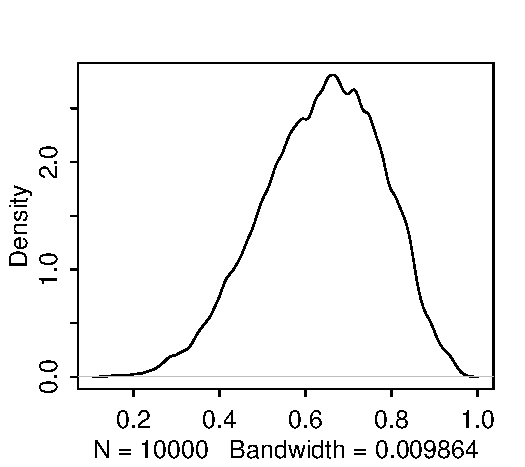
\includegraphics[scale=0.7]{pics/posteriorTossGrid.pdf}
	\end{figure} 
 




\item We can see that the estimated density is very similar to to ideal posterior we computed via
grid approximation in previous class.


 
\end{itemize}



} 

\end{frame}


\begin{frame}[fragile]{Sampling from the theoretical posterior}
\scriptsize{
\begin{itemize}

\item We could get the same results by sampling from the theoretical posterior using the beta distribution: 

\begin{verbatim}
teo.samples<-rbeta(1e4,7,4)
dens(teo.samples)
\end{verbatim}



\item We can see that the estimated density is very similar to the theoretical posterior obtained from the beta distribution:


   \begin{figure}[h!]
	\centering
	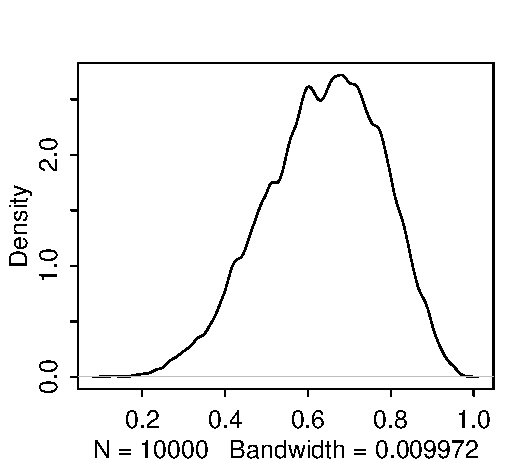
\includegraphics[scale=0.6]{pics/posteriorTossBeta.pdf}
	\end{figure} 


	\item However, we should keep in mind that for complex models we will not have access to the posterior closed form, so it is better to get used to working with samples.
\end{itemize}



} 

\end{frame}

\begin{frame}[fragile]{Intervals of defined boundaries}
\scriptsize{
\begin{itemize}

\item Suppose I ask you for the posterior probability that the proportion of water is less than 0.5. 

\item We could calculate this from the theoretical posterior:

\begin{verbatim}
> pbeta(0.5,7,4)
[1] 0.171875
\end{verbatim}



\item Or alternatively we could calculate it from the grid-approximate posterior by adding up all of the probabilities where the corresponding parameter value is less than 0.5.

\begin{verbatim}
> sum( posterior[ p_grid < 0.5 ] )
[1] 0.1718746
\end{verbatim}


\item So about 17\% of the posterior probability is below 0.5.

\end{itemize}



} 

\end{frame}



\begin{frame}{Intervals of defined boundaries}
\scriptsize{

   \begin{figure}[h!]
	\centering
	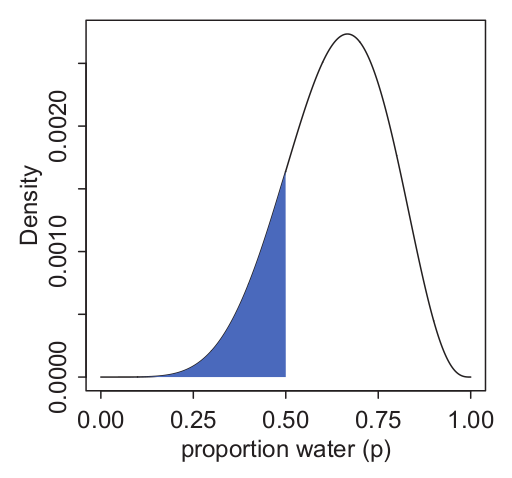
\includegraphics[scale=0.45]{pics/interval1.png}
	\end{figure} 




} 

\end{frame}


\begin{frame}[fragile]{Intervals of defined boundaries}
\scriptsize{
\begin{itemize}

\item Now, let's perform the same calculation, using samples from the posterior.

\item Recall than in more complex models neither a grid-approximation nor a closed-form posterior will be available.

\item All we have to do is add up all samples less than 0.5 and divide the resulting count by the total number of samples.

\begin{verbatim}
> sum( samples < 0.5 ) / 1e4
[1] 0.1752 
\end{verbatim}


\item In R, the condition \verb+samples < 0.5+ returns a logical vector, so since R treats TRUE values as 1, \verb+sum+ will count all the samples satisfying the condition.

\end{itemize}



} 

\end{frame}


\begin{frame}[fragile]{Intervals of defined boundaries}
\scriptsize{
\begin{itemize}

\item Now, we can ask our sample how much posterior probability lies between 0.5 and 0.75.

\begin{verbatim}
> sum( samples > 0.5 & samples < 0.75 ) / 1e4
[1] 0.6043
\end{verbatim}

\item So about 61\% of the posterior probability lies between 0.5 and 0.75.

\item Let's validate this result using the exact posterior:

\begin{verbatim}
> pbeta(0.75,7,4)-pbeta(0.5,7,4)
[1] 0.6040001
\end{verbatim}

\end{itemize}



} 

\end{frame}

\begin{frame}{Intervals of defined boundaries}
\scriptsize{

   \begin{figure}[h!]
	\centering
	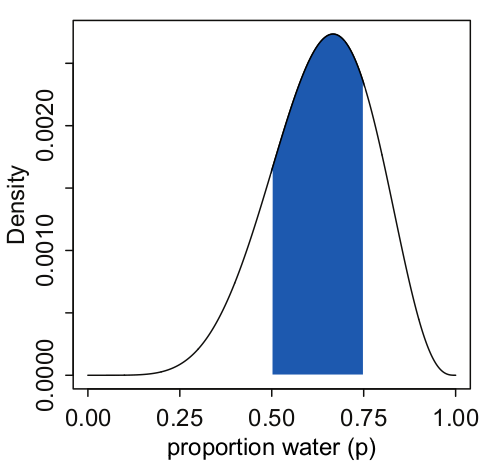
\includegraphics[scale=0.45]{pics/interval2.png}
	\end{figure} 




} 

\end{frame}


\begin{frame}[fragile]{Intervals of defined boundaries}
\scriptsize{
\begin{itemize}

\item The intervals of posterior probability we are working with are called \textbf{credible interval}.

\item They resemble very much the confidence intervals seen in previous lectures on frequentist inference.

\item The interpretations are very different though.

\item A confidence interval is a range that contains the true parameter with a certain chance after infinitely repeating the data sampling experiment.

\item In contrast, a credible interval is a range of values that we believe our parameter can take with a certain probability according to both our prior beliefs and the evidence given by the data.

\end{itemize}



} 

\end{frame}


\begin{frame}{Conclusions}
\scriptsize{

\begin{itemize}
\item Blablaag
\end{itemize}


} 
\end{frame}


%%%%%%%%%%%%%%%%%%%%%%%%%%%
\begin{frame}[allowframebreaks]\scriptsize
\frametitle{References}
\bibliography{bio}
\bibliographystyle{apalike}
%\bibliographystyle{flexbib}
\end{frame}  









%%%%%%%%%%%%%%%%%%%%%%%%%%%

\end{document}
